% Created 2018-11-23 Fri 17:18
% Intended LaTeX compiler: pdflatex
\documentclass[11pt]{article}
\usepackage[utf8]{inputenc}
\usepackage[T1]{fontenc}
\usepackage{graphicx}
\usepackage{grffile}
\usepackage{longtable}
\usepackage{wrapfig}
\usepackage{rotating}
\usepackage[normalem]{ulem}
\usepackage{amsmath}
\usepackage{textcomp}
\usepackage{amssymb}
\usepackage{capt-of}
\usepackage{hyperref}
\author{Kyle Cotton}
\date{\today}
\title{}
\hypersetup{
 pdfauthor={Kyle Cotton},
 pdftitle={},
 pdfkeywords={},
 pdfsubject={},
 pdfcreator={Emacs 26.1 (Org mode 9.1.9)}, 
 pdflang={English}}
\begin{document}

\begin{titlepage}
\begin{center}
{\Large Informatics 1A \par}
\vspace{2cm}
{\Large HASKELL PROGRAMMING COMPETITION \par}
\vspace{2cm}
BY \par
\vspace{2cm}
{\Large KYLE COTTON\\YANNIK NELSON\\DYLAN LYONS\\JASPER KETTEL \par}
\vspace{2cm}
{\large May 18th 2017}
\end{center}
\vfill
\end{titlepage}

\tableofcontents

\section{Inf1-Competition}
\label{sec:orgc84694a}
\subsection{Game of Life}
\label{sec:org2b1e5bb}
Our team has decided to make an improved version of Conan's Game of Life entirely in Haskell.
The code features both two and three dimensional real time rendering; using a team built 3D rendering algorithm.

\subsection{Images of the Program}
\label{sec:org0ce0736}
\subsubsection{3D Version}
\label{sec:orga3a9844}

\begin{center}
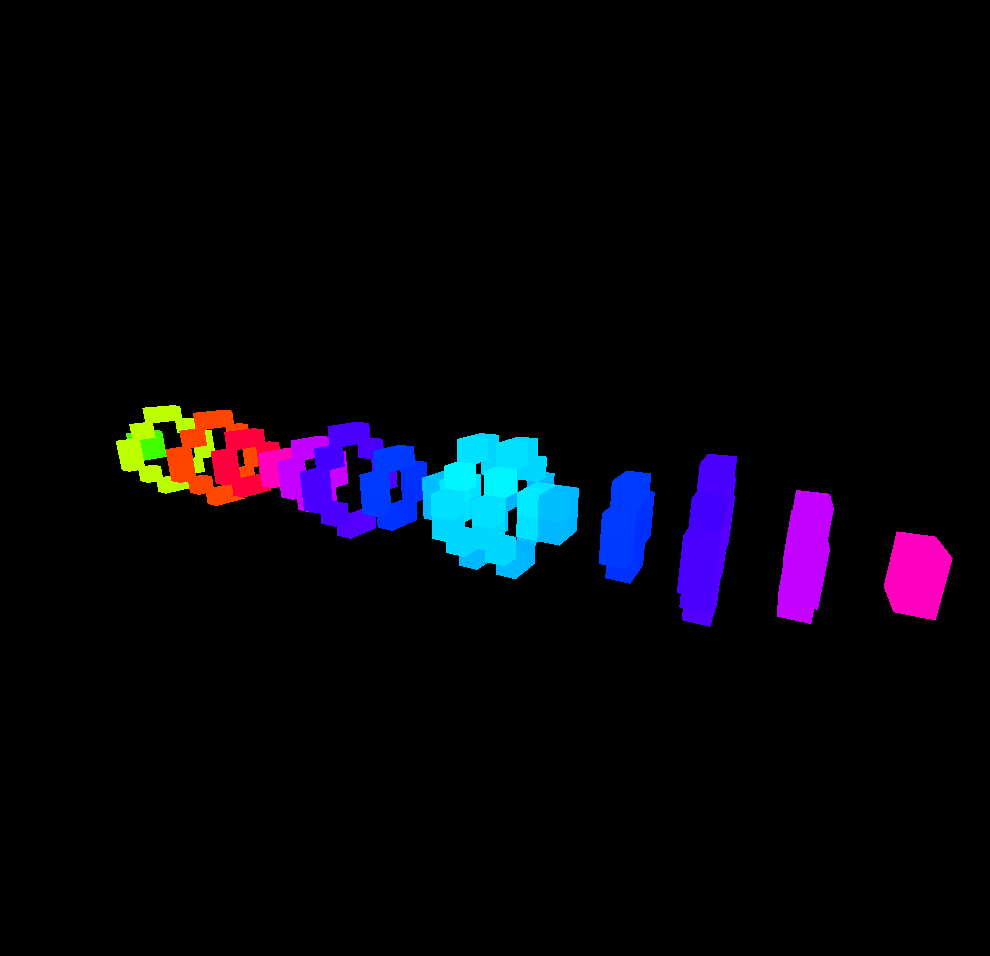
\includegraphics[width=.9\linewidth]{img/1-3.png}
\end{center}

\begin{center}
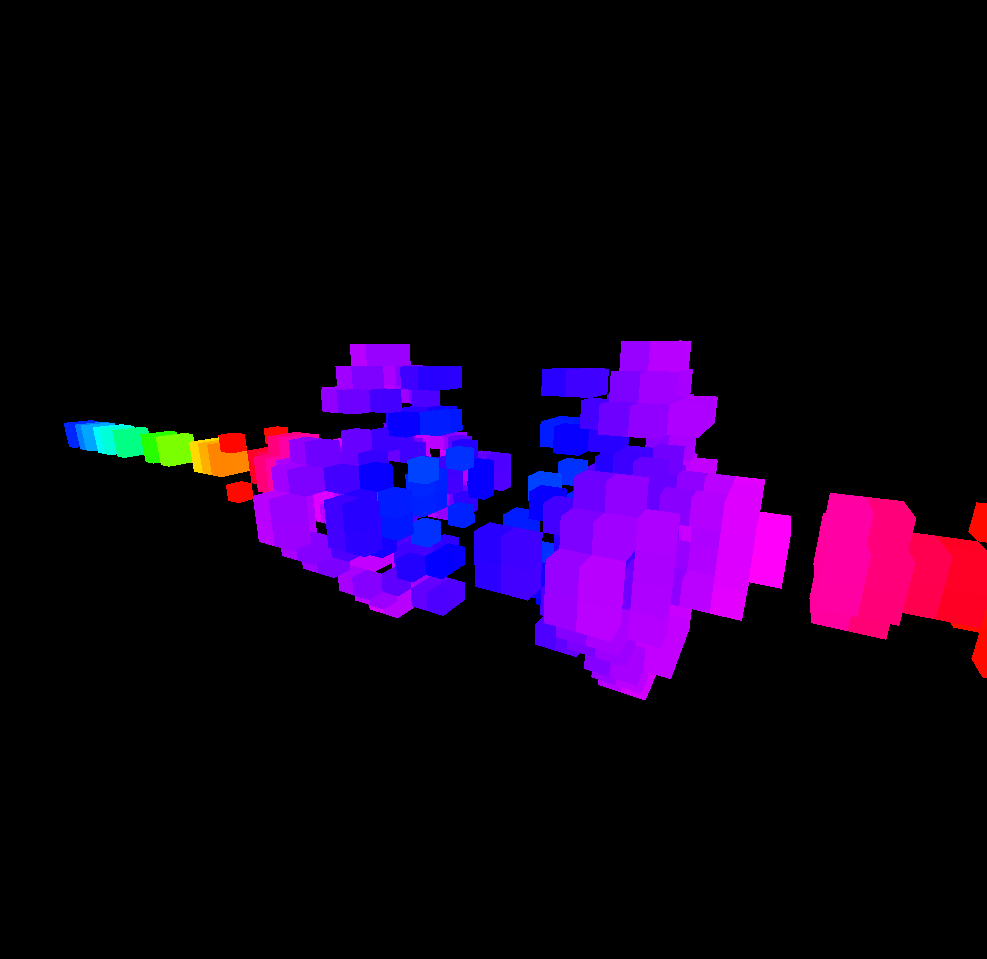
\includegraphics[width=.9\linewidth]{img/2-3.png}
\end{center}

\begin{center}
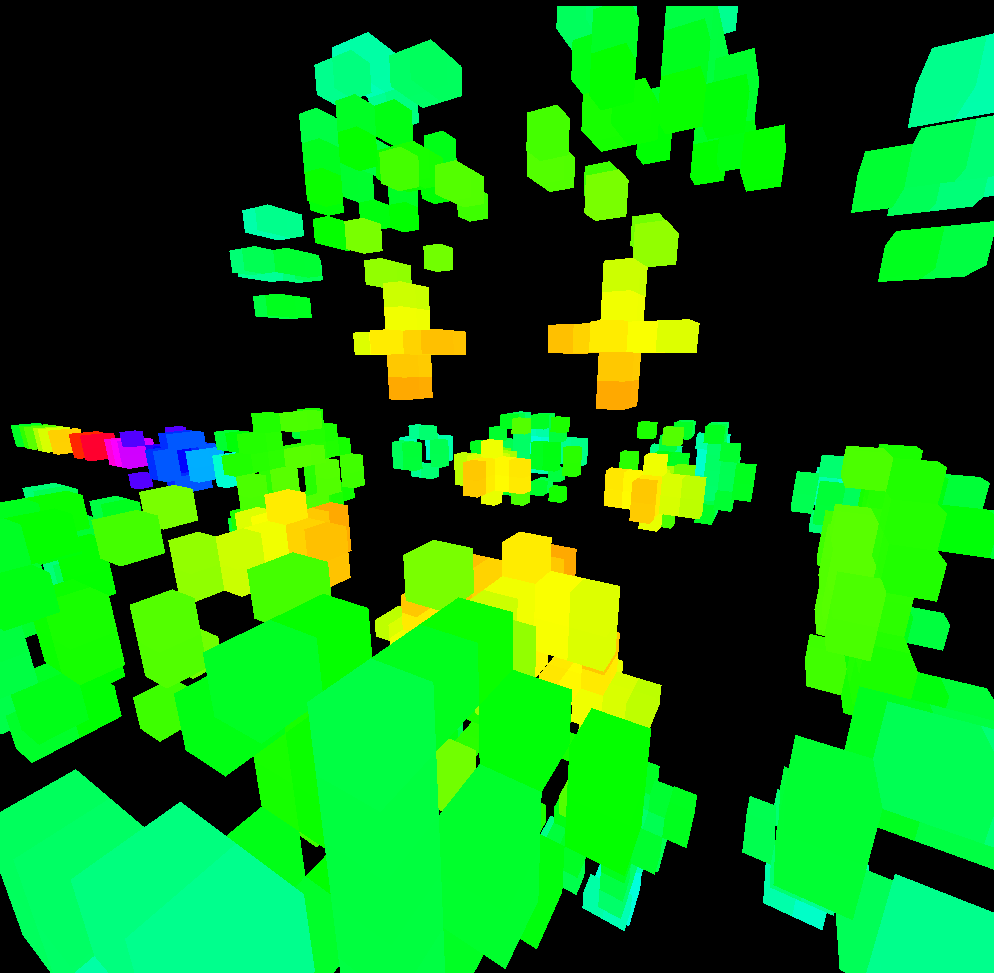
\includegraphics[width=.9\linewidth]{img/3-3.png}
\end{center}

\begin{center}
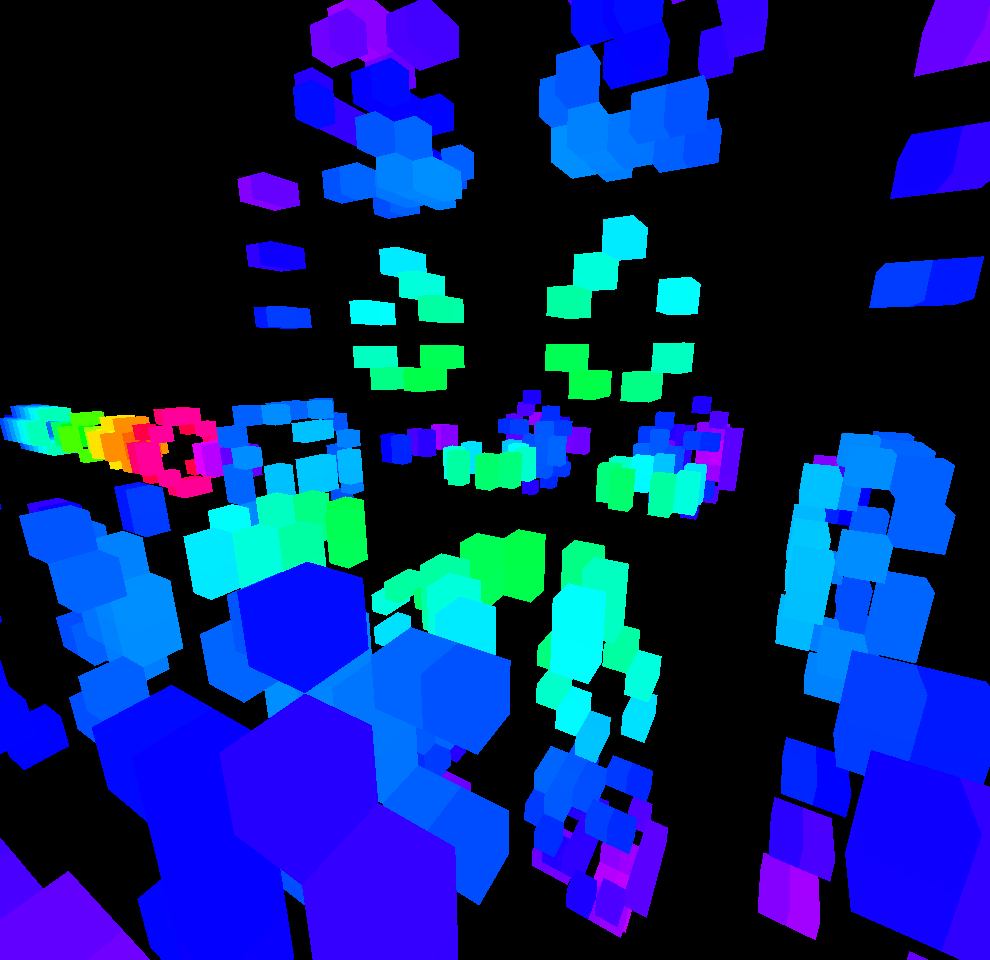
\includegraphics[width=.9\linewidth]{img/4-3.png}
\end{center}

\begin{center}
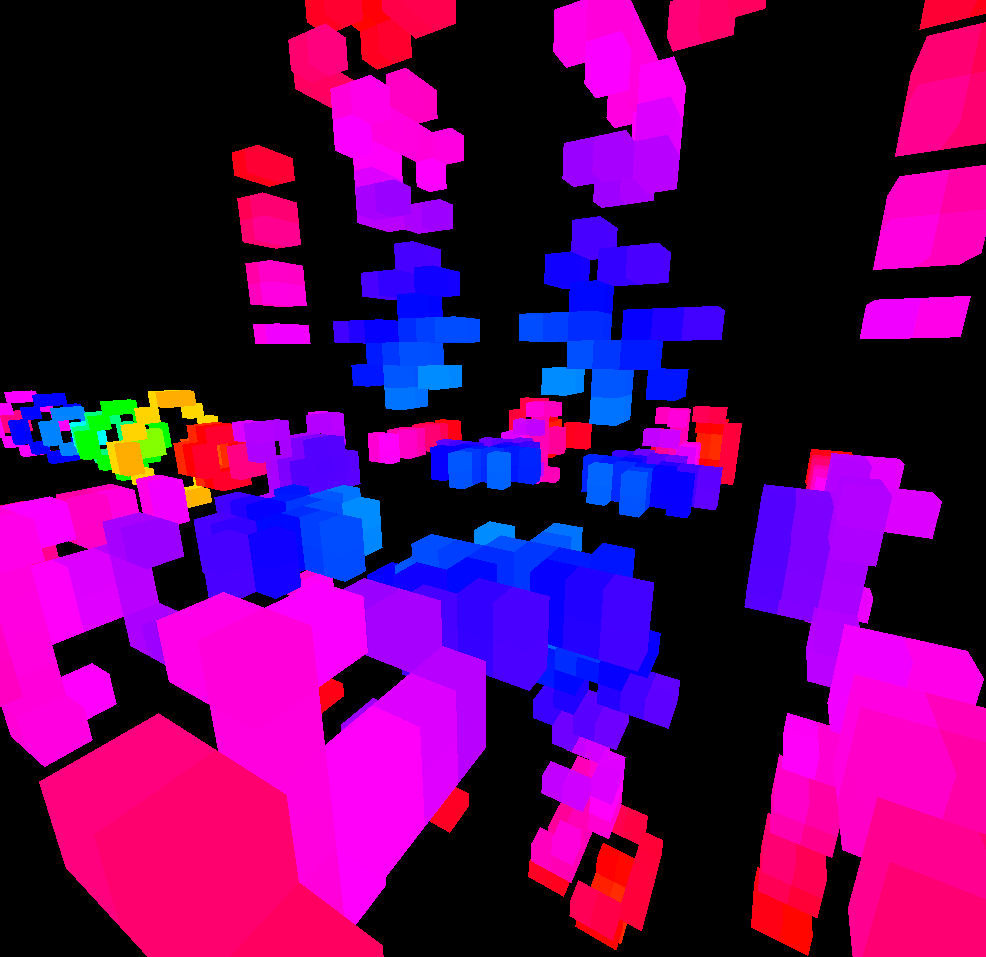
\includegraphics[width=.9\linewidth]{img/5-3.png}
\end{center}

\begin{center}
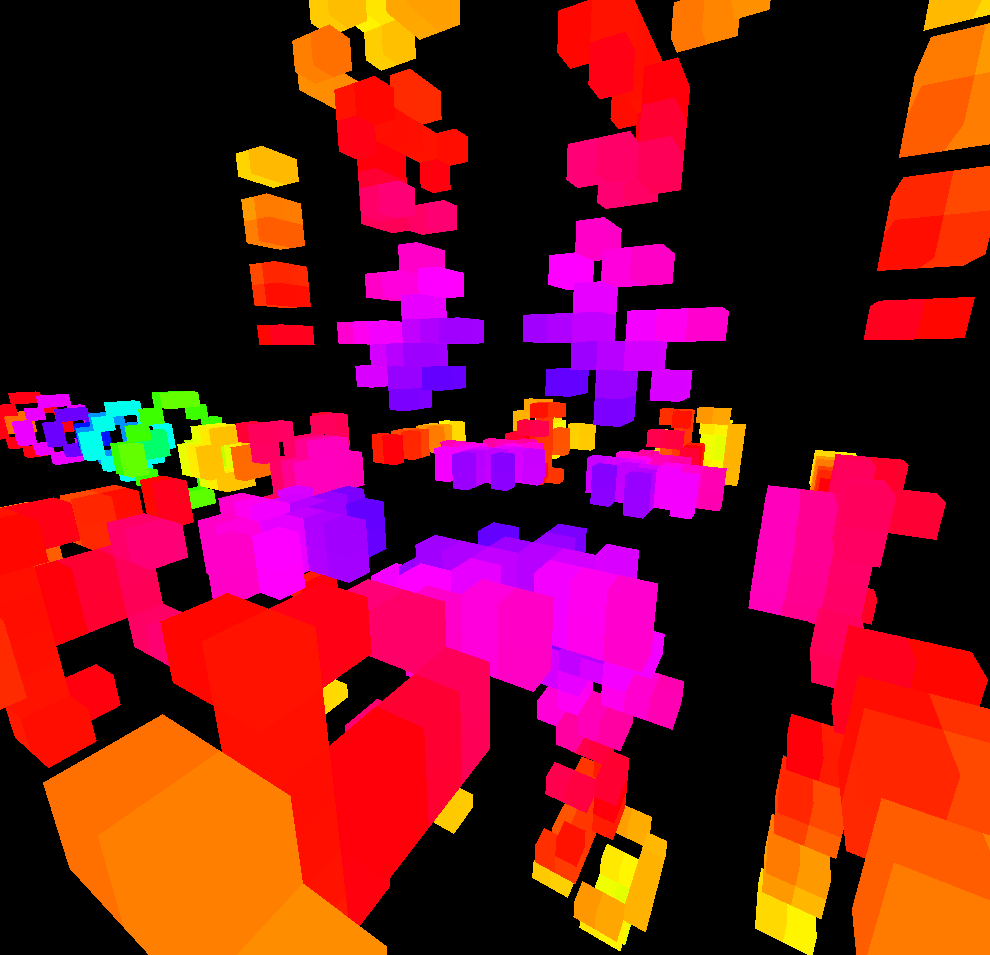
\includegraphics[width=.9\linewidth]{img/6-3.png}
\end{center}

\begin{center}
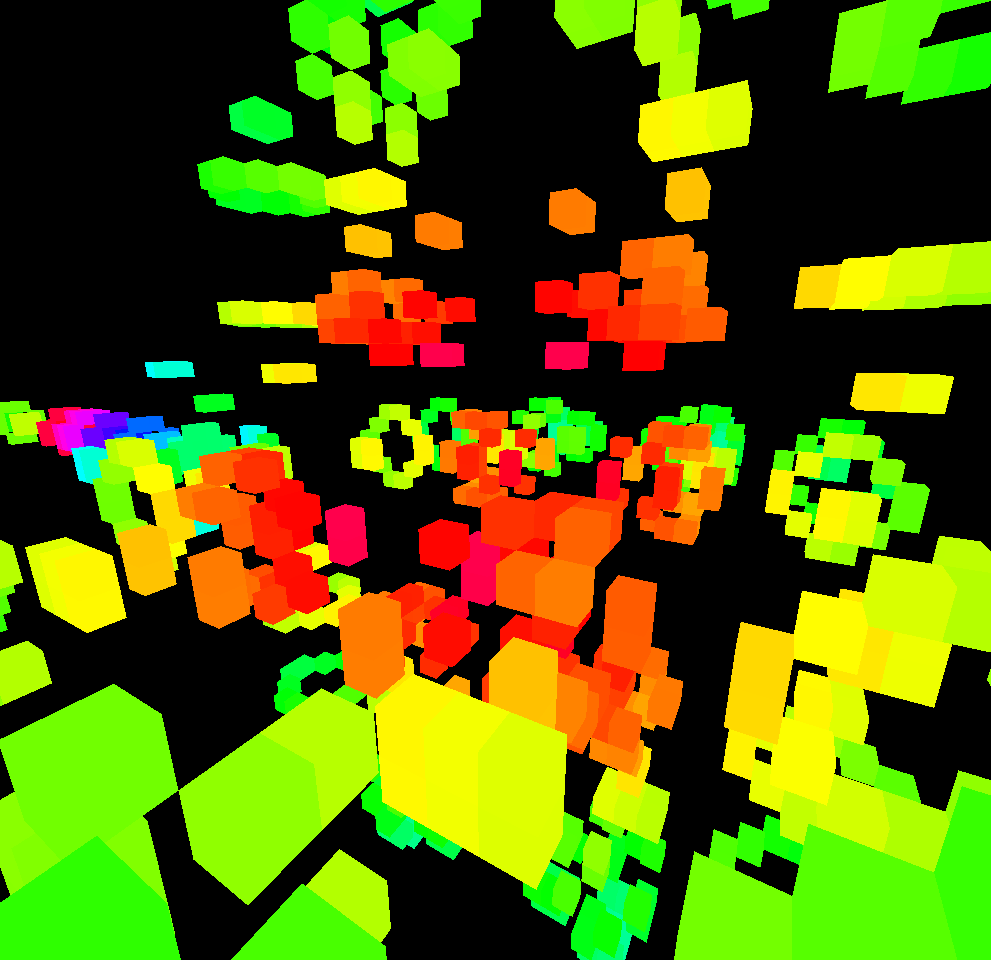
\includegraphics[width=.9\linewidth]{img/7-3.png}
\end{center}
\end{document}
